\documentclass[a4paper, 12pt]{article}
\usepackage[a4paper,top=1.5cm, bottom=1.5cm, left=1cm, right=1cm]{geometry}
\usepackage{cmap}					
\usepackage{mathtext} 				
\usepackage[T2A]{fontenc}			
\usepackage[utf8]{inputenc}			
\usepackage[english,russian]{babel}
\usepackage{multirow}
\usepackage{graphicx}
\usepackage{wrapfig}
\usepackage{tabularx}
\usepackage{float}
\usepackage{wrapfig}
\usepackage{longtable}
\usepackage{hyperref}
\hypersetup{colorlinks=true,urlcolor=blue}
\usepackage[rgb]{xcolor}
\usepackage{amsmath,amsfonts,amssymb,amsthm,mathtools} 
\usepackage{icomma} 
\usepackage{euscript}
\usepackage{mathrsfs}
\usepackage{enumerate}
\usepackage{caption}
\mathtoolsset{showonlyrefs=true}
\usepackage{subcaption}
\usepackage[europeanresistors, americaninductors]{circuitikz}
\DeclareMathOperator{\sgn}{\mathop{sgn}}
\newcommand*{\hm}[1]{#1\nobreak\discretionary{}
	{\hbox{$\mathsurround=0pt #1$}}{}}

\begin{document}

\newgeometry{left=2cm, right=2cm, top=2cm, bottom=1cm,
             bindingoffset=0cm}

\begin{titlepage}
    \begin{center}
        \vspace*{5cm}
        \Huge МФТИ
        \vspace*{2cm}\\
        \LARGE \textbf{Вопрос по выбору}
        \\\vspace*{0.25cm}
        
        \noindent\rule{\textwidth}{1pt}
        \vspace*{-0.25cm}
        
        \huge \textbf{Кумулятивный эффект в жидкости. Падение капли
                      в воду.}
        \noindent\rule{\textwidth}{1pt}

        \vfill

        \begin{flushright}
            \begin{minipage}{.4\textwidth}
            \Large Выполнили: \\ Манро Эйден      \\ (Б01-308) 
                              \\ Солодилов Михаил \\ (Б01-307)
            \end{minipage}
        \end{flushright}
        
        \vfill

        \normalsize Долгопрудный \\2024
    \end{center}
\end{titlepage}

\restoregeometry

\begin{center}
    \section*{Введение}
\end{center}

\noindent \textbf{Цель работы:}
исследовать явление появления кумулятивной струи при падении капли
воды в воду. Исследование зависимости параметров струи от параметров
сосуда и высоты падения капли.

\bigskip

\noindent \textbf{Оборудование:}
сосуд с водой, линейка, штатив, (что-то капающее)

\bigskip

Кумулятивный эффект, эффект Манро (англ. Munroe effect) -- явление
концентрации энергии в одном направлении или в определённом месте.

\begin{figure}[H]
    \begin{subfigure}{0.3\textwidth}
        \centering
        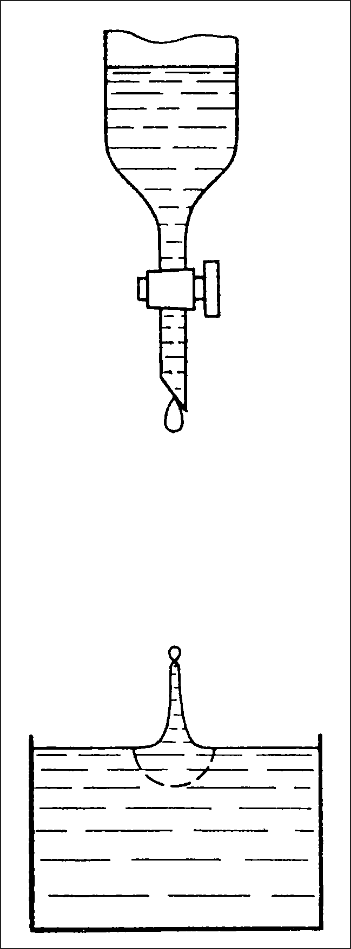
\includegraphics[width=0.5\textwidth]{img/Experiment Scheme.png}
        \caption*{Установка}
    \end{subfigure}%
    \begin{subfigure}{0.5\textwidth}
        \centering
        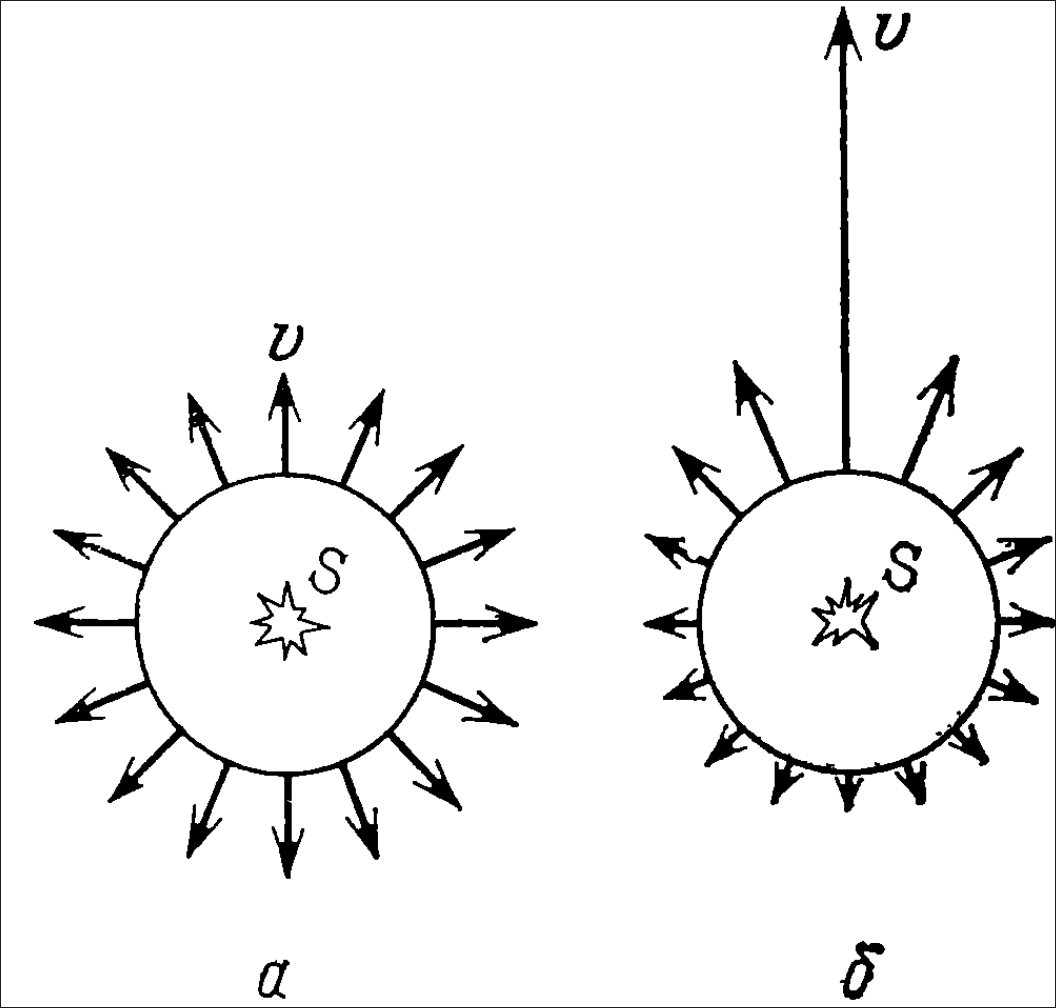
\includegraphics[width=0.7\textwidth]{img/Cumulative effect.png}
        \caption*{\\а -- сферически-симметричный взрыв.\\
                 б -- энергия взрыва сконцентрирована в одном
                 направлении.}
    \end{subfigure}
\end{figure}

Обычно о нём говоярт в очень быстро происходящих процессах, например,
взрывах, но его также можно встретить и в повседневной жизни.
Когда морские волны врезаются в берег, возникает вертикальная
кумулятивная струя. В этой работе мы будем исследовать появление такой
струи при падении капли в воду.

\begin{center}
    \item \section*{Теория}
\end{center}

Весь процесс падения капли можно разделить на 3 этапа:

\bigskip

\begin{enumerate}
    \item Падение капли.
    \item Образование полусферического углубления в жидкости.
    \item Схлопывание углубления и появление кумулятивной струи.
\end{enumerate}

\bigskip

Энергия падении капли выражается следующим образом:

\begin{equation}
    E_k = mgh = \frac{mv^2}{2} = \frac{4}{3}\pi{r^3}{\rho}gh,
\end{equation}

где $r$ -- радиус капли, $h$ -- высота её падения.
Во время образования углубления, энергия капли тратится на образование
поверхности воды и на работу против силы Архимеда:

\begin{equation}
    A_\sigma = \pi{\sigma}R^2,
\end{equation}

\begin{equation}
    A_\text{арх} = \int_{0}^{R} \frac{1}{3}{\pi}{\rho}gy^2(3R-y)dy = 
    \frac{1}{4}\pi{\rho}gR^4
\end{equation}

где $R$ -- радиус углубления.
Суммарная работа получаеся:

\begin{equation}
    A = \pi\sigma{R^2} + \frac{1}{4}\pi{\rho}gR^4.
\end{equation}

Если приравнять её к энергии капли получим:

\begin{equation}
    R = \left [\left (\frac{4\sigma^2}{\rho^2g^2} +
               \frac{16}{3}r^3h \right )^\frac{1}{2}
               - \frac{2\sigma}{\rho{g}} \right ] ^ \frac{1}{2}.
\end{equation}

% \bigskip

Далее вылетает кумулятивная струя. Будем считать, что она имеет форму
цилиндра. Энергия, запасённая в нашем углублении при его схлопывании
тратится на образование столба жидкости и преодоление силы тяжести.

\begin{equation}
    A_\sigma = 2\pi{r_c}l\sigma,
\end{equation}

где $r_c$ -- радиус струи, а $l$ -- её длина.

\begin{equation}
    A_\text{тяж} = \int_{0}^{l} \pi{r_c^2}\rho{g}ydy =
                   \frac{1}{2}\pi{r_c^2}l^2\rho{g}.
\end{equation}

Суммарная работа получается:

\begin{equation}
    A = 2\pi{r_c}l + \frac{1}{2}\pi{r_c^2}l^2\rho{g}.
\end{equation}

Приравняв это к энергии капли найдем параметры струи:

\begin{equation}
    r_cl = \left (\frac{4\sigma^2}{\rho^2g^2} + \frac{8}{3}
                  r^3h \right ) ^ \frac{1}{2} - \frac{2\sigma}{\rho{g}}.
\end{equation}



\end{document}